\label{bg/parallel_computing}
\subsection {What is Parallel Computing}
Parallel Computing is the simultaneous use of multiple computing resources such as processors and memory to solve a computational problem \citep{Barney:16}. Parallel computing is based on the principle of breaking a large problem into smaller problems and solving these smaller problems concurrently on multiple processors.

\subsection{Why Parallelism}
\begin{itemize}
	\item There are physical limit of hardware components how fast they can run
	\item Large application demands more memory and computation time
	\item There are problems that demand real-time constraint
\end{itemize}

\subsection{Sequential vs. Parallel execution}

\subsubsection{Sequential execution}
Single sequence of instructions is executed one at time by a single processing unit on a single sequence of data \citep{Akl2009}. Figure \ref{fig:sequential-processing} shows a problem consists of a set of instructions \textbf{(t1, t2, ..., tN)} that are executed by the processor in a sequential manner.

\begin{figure}[!htb]
  \center
  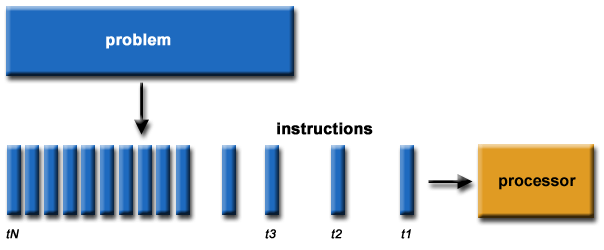
\includegraphics[width=\linewidth]{figs/serialProblem.png}
  \caption{Sequential processing where instructions (t1, t2, ..., tN) of a problem are executed by a single processors sequentially. \citep{Barney:16}}
  \label{fig:sequential-processing}
  \center
\end{figure}

\subsubsection{Parallel execution}
In parallel execution a problem can be broken into smaller sub-problems and two or more processors can work on it simultaneously. During this phase the processors may need to communicate with each other to exchange partial results. At the end of the computation the interim results from each processors must be combined to form the final solution to the original problem. Figure \ref{fig:parallel-processing} shows a problem is broken down into sub-problems each of which then consist of a set of instructions \textbf{(t1, t2, ..., tN)} that are executed by different processors in parallel.

\begin{figure}[!htb]
  \center
  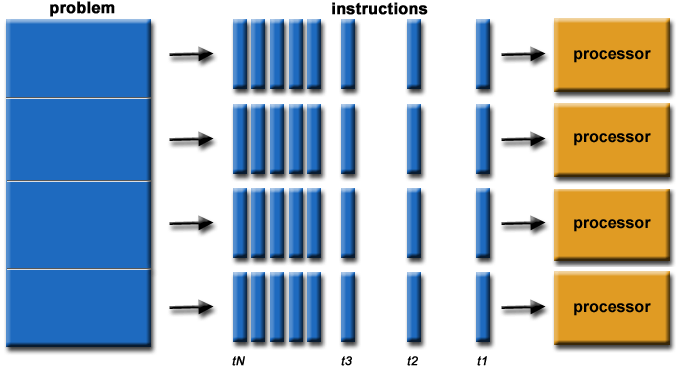
\includegraphics[width=\linewidth]{figs/parallelProblem.png}
  \caption{Parallel processing where a problem is broken down into a number of sub-problems with their own set of instructions (t1, t2, ..., tN) that can be executed in parallel by different processors. \citep{Barney:16}}
  \label{fig:parallel-processing}
  \center
\end{figure}

\subsection{Types of Parallelism}

\paragraph{Data parallelism}
In Data parallelism the input data is divided among different processors. The same task runs on different parts of the data in parallel. Data parallelism is a consequence of single operations that is being applied on multiple data items

\paragraph{Task Parallelism}
In Task parallelism different tasks run on the same data. In this model, parallelism is expressed by a task graph. A task graph can be either trivial or nontrivial. The correlation among the tasks are utilised to promote locality or to minimise interaction costs. This model is enforced to solve problems in which the quantity of data associated with the tasks is huge compared to the number of computation associated with them. The tasks are assigned to help improve the cost of data movement among different tasks.

\paragraph{Hybrid data/task parallelism}
A parallel pipeline of tasks, each of which might be data parallel

\subsection{Flynn's Classical Taxonomy}
This is known as one of the earliest classification of computers and programs created by Michael J. Flynn \citep{Barney:16}. Flynn classified programs and computers on instructions stream and data stream.

\begin{description}
\item [SISD] {Single Instruction Single Data}

Only one instruction is being acted on by the CPU during one clock cycle and only one data stream is being used as input.

\item [SIMD] Single Instruction Multiple Data

All processing unit execute same instruction at any given clock cycle but each processing using act upon different data input.

\item [MISD] Multiple Instructions Single Data

Each processing unit execute separate instruction stream independently on a single data stream.

\item [MIMD] Multiple Instructions Multiple Data

Each processor executes different instruction stream and all of them work on different data input stream.
\end{description}

This classification model distinguishes multi-processors computer architecture based on how they can be classified along the two independent dimension of Instruction Steam and Data Stream. There are further classification exist based on multiple data stream. \textbf{Single Program Multiple Data (SPMD)} is a subcategory of MIMD where multiple processors simultaneously execute same program on different data input.\citep{Barney:16}

\subsection{Classification of Parallel Computers}
Parallel computers can be classified based on their hardware supports. 
\begin{itemize}
	\item \textbf{PVP (Parallel Vector Processor)}

PVP systems contain a small number of powerful custom made vector processors with shared memory.
	\item \textbf{SMP   (Symmetric Multiprocessor)}
	
SMP system consist of a number of processors connected through a bus system. Each processor has equal access to memory, I/O etc.
	
	\item \textbf{MPP   (Massively Parallel Processor)}
	
MPP is very large-scale computer system with many processors and physically distributed memory space. This system requires high communication bandwidth and low latency interconnection between processors. It is a tightly couple system.
	
	\item \textbf{COW (Cluster of Workstation)}
	
COW is a low-cost variation of MPP which consist of multiple nodes(a complete workstation) connected by low-cost network. Nodes work together as a single integrated computing resource. This system is loosely coupled and highly extensible. Beowulf cluster falls into this category.
	
	\item \textbf{DSM  (Distributed Shared Memory)}
	
DSM uses special hardware and software extension to support distributed coherent caches. In contrast with SMP system, DSM consist of distributed-memory but hardware and software gives an illusion of shared-memory behaviour.
\end{itemize}
\citep{Perkowski:10}

\subsection{Parallel Computer Memory Architecture}
\paragraph{Shared Memory model}
Multiple processor operate independently but share the same address space. Figure \ref{fig:shared-memory} shows the shared-memory model architecture.

\begin{figure}[!h]
\centering
  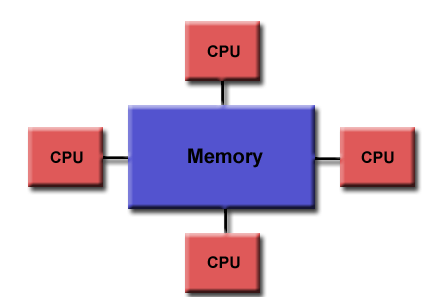
\includegraphics[width=.5\linewidth]{figs/shared-memory.png}
  \caption{A Shared Memory model where multiple CPU is sharing a common memory space. \citep{Barney:16}}
  \label{fig:shared-memory}
\end{figure}

\paragraph{Distributed Memory Model}
Processors have their own local address space. Memory address of one processor do not map to another. A message-passing mechanism is required for data sharing. Figure \ref{fig:distributed-memory} shows the distributed-memory model architecture.

\begin{figure}[!h]
\centering
  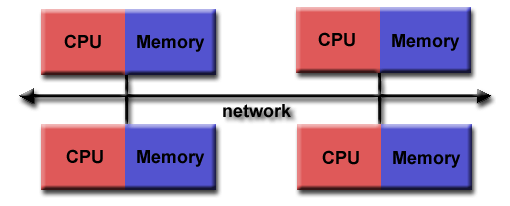
\includegraphics[width=.5\linewidth]{figs/distributed-memory.png}
  \caption{A Distributed Memory model where multiple CPUs have their own memory spaces but connected together with network bus to exchange messages. \citep{Barney:16}}
  \label{fig:distributed-memory}
\end{figure}

\paragraph{Hybrid Model}
Hybrid model is the combination of shared-memory interconnected by network communication that allows distributed-memory access of data resides in another processors global space. Figure \ref{fig:hybrid-memory} show the Hybrid-memory model architecture.

\begin{figure}[!h]
\centering
  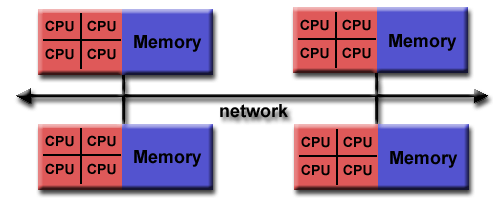
\includegraphics[width=.5\linewidth]{figs/hybrid-memory.png}
  \caption{A Hybrid Memory model where multiple shared-memory systems are interconnected together by a network communication  to exchange messages. \citep{Barney:16}}
  \label{fig:hybrid-memory}
\end{figure}

\citep{Barney:16}
\subsection{Limitation of Parallel Programming}
\subsubsection{Amdahl's Law}
Amdahl's law states that a programs speedup of an algorithm on parallel computing platform is defined by:

\[	S = \frac{1}{(1 - f) + \frac{f}{N}}  \]

Where,
\begin{itemize}
\item \textit{S} is the maximum speedup in execution time of entire task
\item \textit{f} is the percentage of the task that can be parallelise
\item \textit{N} is number of parallel processors 
\end{itemize}

From Amdahl's Law it become apparent that there is limits to the scalability of parallelism. The speedup gain on parallelising a tasks is dependent on the ratio of paralellisable codes \citep{Barney:16}. The graph in Figure \ref{fig:amdahls_law} shows the limit of speed up of parallel execution of code. This Law argued that there exist a  speed up limit; which is $ 1/(1-f) $.

\begin{figure}[!h]
\centering
  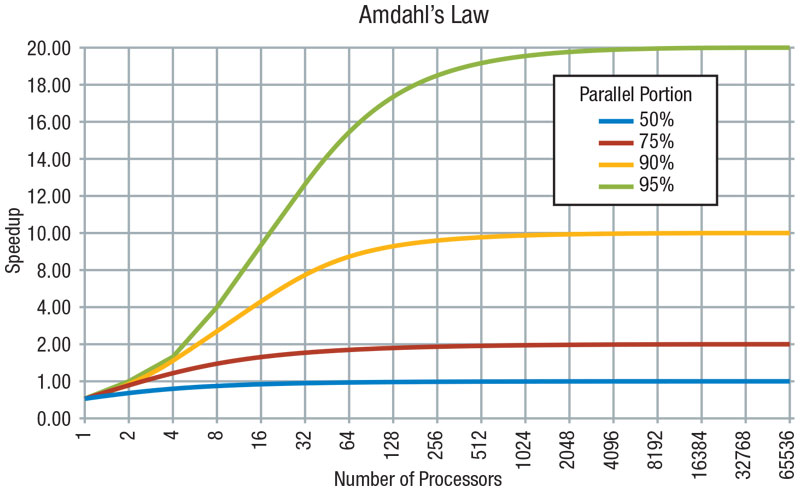
\includegraphics[width=.8\linewidth]{figs/amdahls_law.jpg}
  \caption{Amdahl's Law shows that speedup increases both as a function of the percentage of parallelism and the number of parallel units available. \citep{rtc_amdals:online}}
  \label{fig:amdahls_law}
\end{figure}

\subsubsection{Gustafson's Law}
The problem with Amdahl's law is that, it is assumed that the problem size is fixed for both serial and parallel parts. In an empirical studies by John Gustafson \citep{gustafson:88} showed that when problem size scales up, by scaling up the number of parallel processors the execution time can be kept fixed. The limitation imposed by the serial parts of a program may be countered by increasing the total amount of computation. This is known as Gustafson's law.

Gustafson's law is formulated as:

\[	S = (1 - f) + fN  \]
Where, 
\begin{itemize}
\item \textit{S} is the maximum speedup in execution time of entire task
\item \textit{f} is the percentage of the task that can be parallelise
\item \textit{N} is number of parallel processors 
\end{itemize}

In Figure \ref{fig:speed_up_fixed_scaled} the two models of parallel speedup contrasted and summarised in terms of gains based on fixed-size and scaled sized parallel portion in a program. As described by Amdahl's Law, if a program with \textit{s} serial portion and \textit{p}  parallel portion requires 1 time unit to run on a serial processors then it requires  $ s + p/N$ time unit on \textit{N} parallel processors. Therefor, the overall speed up is $ 1/(s+p/N)$. It is assumed that the parallel portion \textit{p} is fixed. 

In Figure \ref{fig:speedup_scaled} shows if the parallel portion of the program increases(where serial portion is shown as $ s' $ and parallel portion as $ p' $) time requires to run this program on serial processor is $ s' + Np'$ in comparison to running it on \textit{N} parallel processors. Therefore, if the number of processors \textit{N} is increased in proportion to the scaled up parallel portion of the program then the speedup is $ s' + Np'$.

\begin{figure}[!h]
	\begin{subfigure}[b]{\textwidth}
		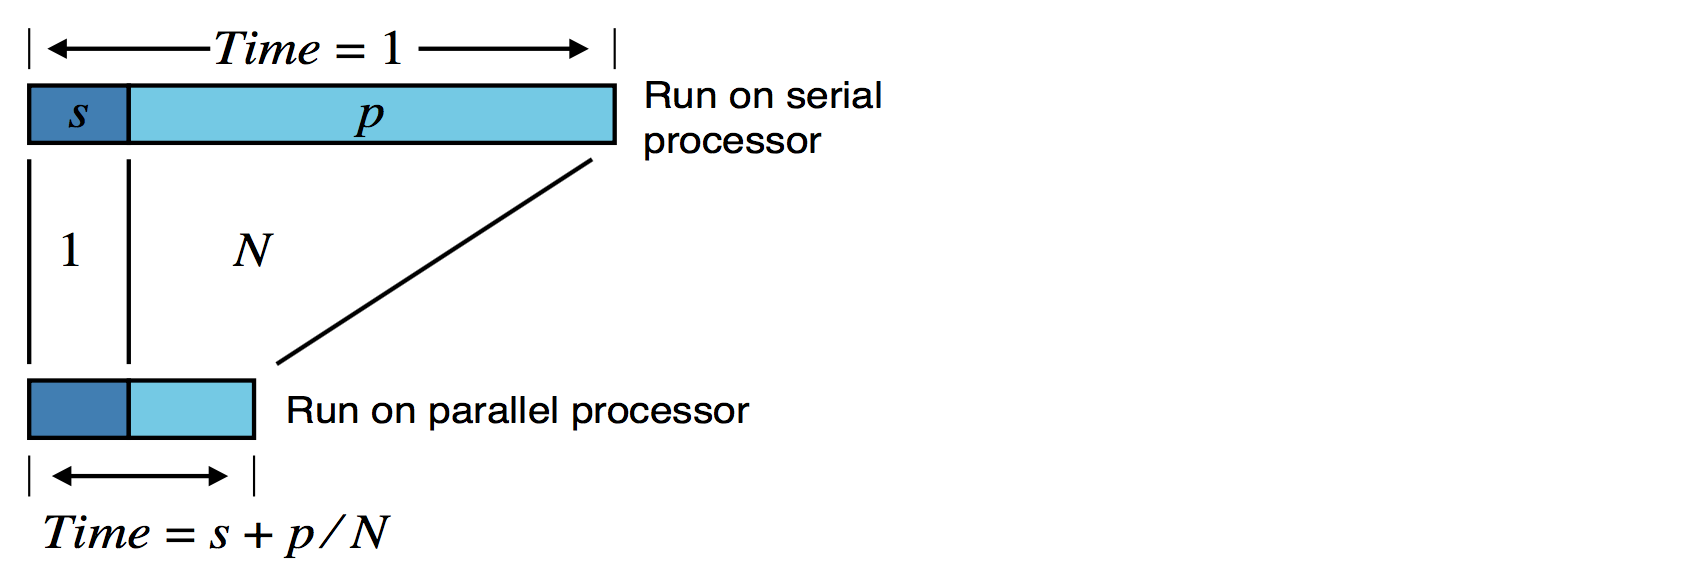
\includegraphics[width= .9 \textwidth]{figs/speedup_fixed.png}
  		\caption{A program with \textit{s} serial portion and parallel portion \textit{p} requires 1 time unit to run on a serial processors and  $ s + p/N$ on \textit{N} parallel processors. Therefor, the overall speed up is $ 1/(s+p/N)$.}
  		\label{fig:speedup_fixed}
	\end{subfigure}
	\begin{subfigure}[b]{\textwidth}
		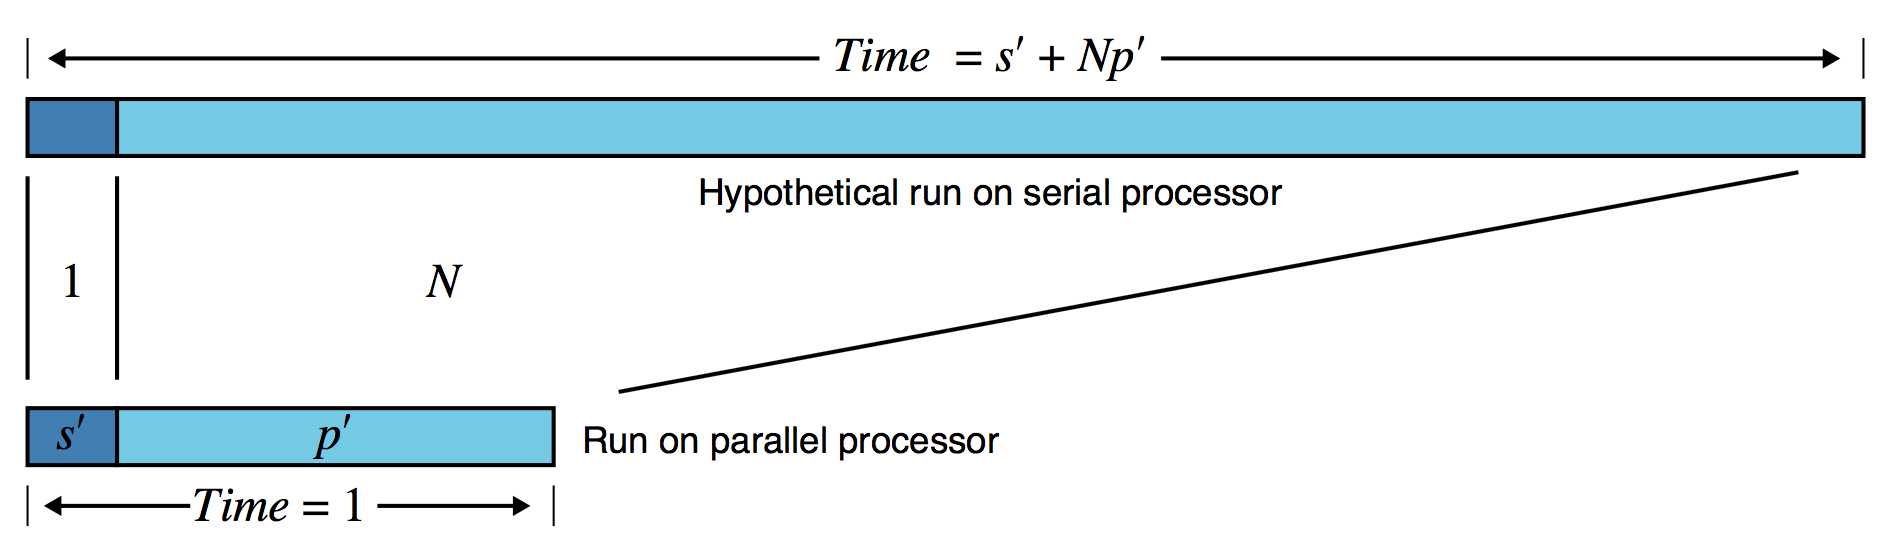
\includegraphics[width=\textwidth]{figs/speedup_scaled.png}
  		\caption{A program with $s'$ serial portion and $p'$ parallel portion requires 1 time unit to run on \textit{N} parallel processors and $ s' + Np'$ unit time on a serial processor. Therefor, the overall speed up is $ (s'+Np')/1$ i.e. $s'+Np'$.}
  		\label{fig:speedup_scaled}
	\end{subfigure}
	\caption{Comparison of speedup of fixed-sized and scaled-sizes parallel portion of a program.}
	\label{fig:speed_up_fixed_scaled}
\end{figure}

\citep{gustafson:88}

\subsection{Application}
Parallel computation many application areas, which include:
\begin{itemize}
	\item Scientific Computing
	\item Simulation
	\item Aerospace
	\item Weather forecasts - Climate changes
	\item Astronomy - Planetary movement
	\item Big Data and Data mining
\end{itemize}

\citep{Barney:16}